% Compile with XeLaTeX, TeXLive 2013 or more recent
\documentclass{beamer}

% Base packages
\usepackage{fontspec}

\usepackage{xunicode}
\usepackage{xltxtra}

\usepackage{amsfonts}
\usepackage{amsmath}
\usepackage{longtable}
\usepackage{csquotes}
\usepackage{standalone}

\usepackage{graphicx}
\graphicspath{{./images/}}

\usepackage{tikz}
\usetikzlibrary{arrows,decorations.pathmorphing,backgrounds,positioning,fit,petri}

\usepackage{listings}
\lstset{language=C, basicstyle=\ttfamily, breaklines=true, keepspaces=true, keywordstyle=\color{blue}}

% Setup Russian hyphenation
\usepackage{polyglossia}
\setdefaultlanguage[spelling=modern]{russian} % for polyglossia
\setotherlanguage{english} % for polyglossia

% Setup fonts
\newfontfamily\russianfont{CMU Serif}
\setromanfont{CMU Serif}
\setsansfont{CMU Sans Serif}
\setmonofont{CMU Typewriter Text}

% Be able to insert hyperlinks
\usepackage{hyperref}
\hypersetup{colorlinks=true, linkcolor=black, filecolor=black, citecolor=black, urlcolor=blue , pdfauthor=Evgeny Yulyugin <yulyugin@gmail.com>, pdftitle=Параллельное программирование}
% \usepackage{url}

% Misc optional packages
\usepackage{underscore}
\usepackage{amsthm}

% A new command to mark not done places
\newcommand{\todo}[1][]{{\color{red}TODO\ #1}}

\newcommand{\abbr}{\textit{англ.}\ }

\subtitle{Курс «Параллельное программирование»}
\subject{Lecture}
\author[Евгений Юлюгин]{Евгений Юлюгин \\ \small{\href{mailto:yulyugin@gmail.com}{yulyugin@gmail.com}}}
\date{\today}
\pgfdeclareimage[height=0.5cm]{mipt-logo}{../common/mipt.png}
\logo{\pgfuseimage{mipt-logo}}

\typeout{Copyright 2014 Evgeny Yulyugin}

\usetheme{Berlin}
\setbeamertemplate{navigation symbols}{}%remove navigation symbols


\title{Области применения многопроцессорных систем. Примеры многопроцессорных и распределенных систем.}

\begin{document}

\begin{frame}
\titlepage
\end{frame}

\section*{Обзор}

\begin{frame}{На этой лекции}
\tableofcontents
\end{frame}

\section{Область применения}

\begin{frame}{Область применения}
\begin{itemize}
    \item Моделирование и анализ транспортных потоков,
    \item Разработка лекарственных препаратов,
    \item Прогнозирование погоды,
    \item Поисковые системы,
    \item Распознование изображений,
    \item Банковский сектор,
    \item Наука.
\end{itemize}
\end{frame}

\begin{frame}{Кто использует МВС?}
\begin{figure}[htpb]
\pause
\begin{minipage}[htpb]{0.3\textwidth}
\center{
\includegraphics[width=\textwidth]{google-logo}}
\end{minipage}
\pause
\hspace*{0.05\textwidth}
\begin{minipage}[htpb]{0.25\textwidth}
\center{
\includegraphics[width=\textwidth]{intel-logo}}
\end{minipage}
\pause
\vfill
\begin{minipage}[htpb]{0.3\textwidth}
\center{
\includegraphics[width=\textwidth]{nasa-logo}}
\end{minipage}
\pause
\begin{minipage}[htpb]{0.3\textwidth}
\center{
\includegraphics[width=\textwidth]{sberbank-logo}}
\end{minipage}
\pause
\begin{minipage}[htpb]{0.3\textwidth}
\center{
\includegraphics[width=\textwidth]{common/mipt}}
\end{minipage}
\end{figure}
\end{frame}

\section{Типы МВС}

\begin{frame}{Типы МВС}
Наиболее распространенные типы многопроцессорных вычислительных систем:
\begin{itemize}
    \item Системы высокой надежности,
    \item Системы для высокопроизводительных вычислений,
    \item Многопоточные системы.
\end{itemize}
\end{frame}

\section{Требования}

\begin{frame}{Требование к системе}
\begin{itemize}
    \item Производительность,
    \item Энергопотребление,
    \item Время простоя,
    \item Надежность и отказоустойчивость,
    \item Масштабируемость.
\end{itemize}
\end{frame}

\section{Измерение производительности}

\begin{frame}{MIPS}
IPS (\abbr Instructions Per Second).
\vspace*{0.5cm}

Вариации:
\begin{itemize}
    \item kIPS (\abbr thousand instructions per second),
    \item MIPS (\abbr million instructions per second),
    \item GIPS (\abbr giga instructions per second).
\end{itemize}
\end{frame}

\begin{frame}{FLOPS}
FLOPS (\abbr FLotin Point Operations Per Second).
\vfill
Недостатки:
\begin{itemize}
    \item Не учитывает разрядоность операндов,
    \item Не учитывает другие факторы, не связанные с производительностью
    вычислительного модуля:
    \begin{itemize}
        \item Пропускная способность каналов связи,
        \item Производительность памяти,
        \item Работа кэш-памяти.
    \end{itemize}
\end{itemize}
\vfill
Результаты полученные на одной и той же системе при помощи разных тестов
производительности могут быть разными!
\end{frame}

\begin{frame}{Benchmarks}
Тест производительности (\abbr benchmark).
\vfill
Примеры:
\begin{itemize}
    \item \href{http://www.netlib.org/utk/people/JackDongarra/faq-linpack.html}{Linpack} --- FLOPS,
    \item \href{http://www.spec.org/benchmarks.html}{SPEC CPU} --- MIPS,
    \item \href{http://www.superpi.net}{SuperPI} --- single thread --- время вычислений.
    \item \href{http://www.3dmark.com/}{3DMark} --- GPU performance --- gaming benchmark.
\end{itemize}
\end{frame}

\begin{frame}{TOP500 Supercomputers}
\href{http://top500.org/}{TOP500 Supercomputers}:
\begin{itemize}
    \item Проект запущен в 1993 году;
    \item Актуальный список публикуется дважды в год (в июне и ноябре);
    \item Основой рейтинга являеются реузльтаты исполнения теста Linpack (HPL).
\end{itemize}
\vfill
Измеряемые величины:
\begin{itemize}
    \item RMAX --- Максимальная производительность, полученный при использовании
    тестов Linpack;
    \item RPEAK --- Теоретичекая пиковая производительность системы.
\end{itemize}
\end{frame}

\begin{frame}{Рейтинг}
November 2014:
\begin{table}[htpb]
    \begin{center}
    \begin{tabular}{|l|r|r|r|r|}
    \hline
            &                   &               &   RMAX,       &   RPEAK,      \\
    Rank    &   Location        &   Cores       &   TFLOPS      &   TFLOPS      \\
    \hline
    1       &   China           &   3,120,000   &   33,862.7    &   54,902.4    \\
    \hline
    2       &   United States   &   560,640     &   17,173.2    &   27,112.5    \\
    \hline
    3       &   United States   &   1,572,864   &   10,510.0    &   11,280.4    \\
    \hline
    4       &   Japan           &   705,024     &   8,586.6     &   10,066.3    \\
    \hline
    \multicolumn{5}{c}{...}                                                     \\
    \hline
    23      &   Russia          &   37,120      &   1,849.0     &   2,575.9     \\
    \hline
    \end{tabular}
    \end{center}
\end{table}
\end{frame}

\begin{frame}{История}
\begin{figure}
\center{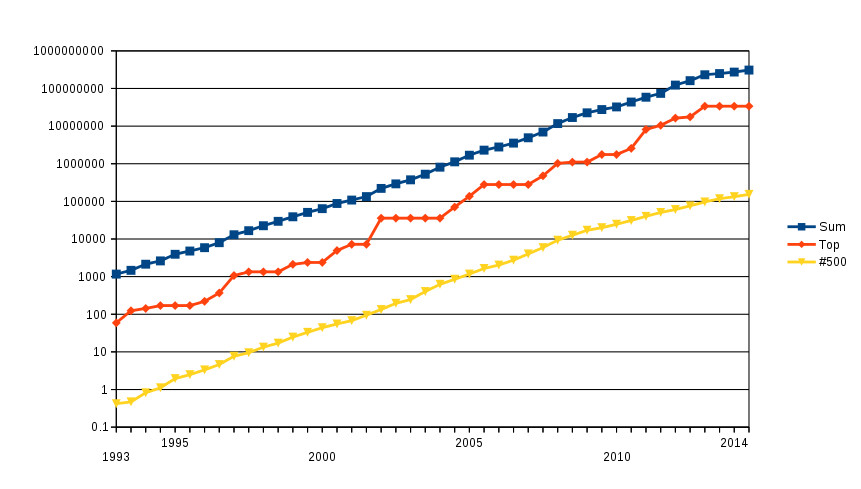
\includegraphics[width=\textwidth]{top500-history}}
\end{figure}
\end{frame}

\begin{frame}{Распределение по странам}
\begin{figure}
\center{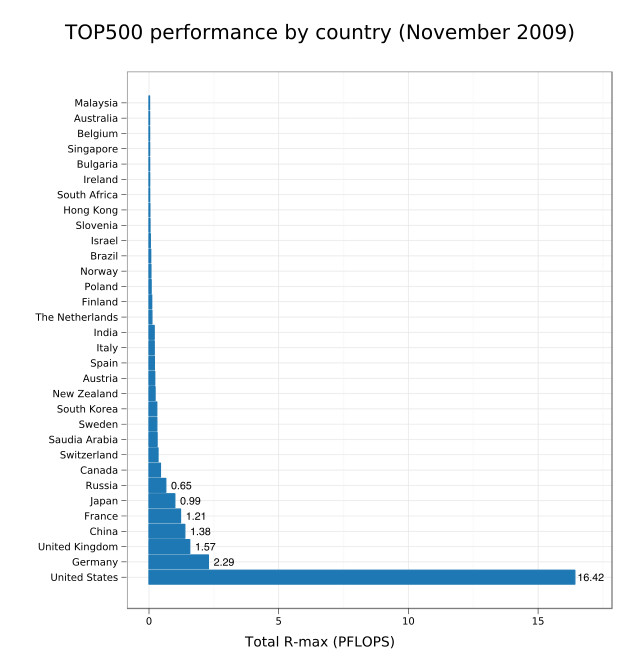
\includegraphics[width=0.6\textwidth]{top500-2009-by-country}}
\end{figure}
\end{frame}

\section{Закон Мура}

\begin{frame}{Закон Мура}
В 1965 году один из основателей Intel --- Гордон Мур --- сформулировал
эмпирическое утверждение:
\vfill
Количество полупроводниковых элементов на кристалле и производительность
процессора удваивается в среднем каждые полтора--два года.
\end{frame}

\begin{frame}{Закон Мура на 2011 год}
\begin{figure}
\center{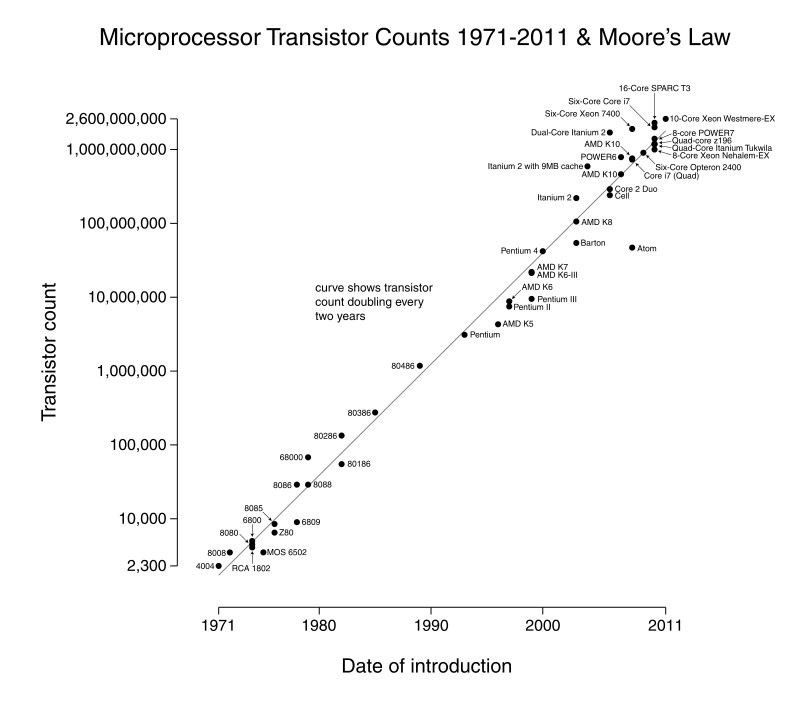
\includegraphics[width=0.7\textwidth]{moores-law-2011}}
\end{figure}
\end{frame}

\begin{frame}{Закон Мура для МП систем}
В 2005 году появились многоядерные процессоры.
\vfill
Удвоение количиства ядер на процессоре происходит каждые полтора--два года.
\end{frame}

\section*{Конец}

\begin{frame}[allowframebreaks]{Рекомендуемая литература}
\begin{thebibliography}{99}
    \bibitem{} \textit{Богданов~А.В., Корхов~В.В., Мареев~В.В., Станкова~Е.Н.}
    Архитектуры и топологии многопроцессорных вычислительных систем. --- М.:
    ИНТУТ.РУ, 2004 --- 176~с. ISBN 5-9556-0018-3.
    \bibitem{} \textit{Таненбаум~Э.} Архитектура компьютера. --- 5-е изд. ---
    СПб.~Питер, 2007 --- 844~c. ISBN 5-469-01274-3.
    \bibitem{} \textit{John L. Hennessy, David A. Patterson} Computer
    Architecture: A Quantitative Approach --- 4th ed. --- 2007 --- 676~p.
    \bibitem{} \textit{Карпов~В.Е.} Введение в распараллеливание алгоритмов и
    программ. --- Компьютерные исследования и моделирование. --- 2010 --- Т.~2
    --- \textnumero~3 --- C.~231--272.
\end{thebibliography}
\end{frame}

\begin{frame}{На следующей лекции}
\begin{itemize}
\ifsbertech
    \item Общие понятия и определения,
    \item Состояние гонки,
    \item Синхронизация,
    \item Ошибки синхронизации.
\fi
\ifmipt
    \item История MPI,
    \item Принцип работы MPI,
    \item Базовые функции MPI,
    \item Компиляция и запуск,
    \item Примеры.
\fi
\end{itemize}
\end{frame}

\begin{frame}

{\huge{Спасибо за внимание!}\par}

\vfill

\tiny{\textit{Замечание}: все торговые марки и логотипы, использованные в данном материале, являются собственностью их владельцев. Представленная здесь точка зрения отражает личное мнение автора, не выступающего от лица какой-либо организации.}

\end{frame}

\end{document}
